% The Results section is dedicated to presenting the actual results (i.e.
% measured and calculated quantities), not to discussing their meaning or
% interpretation. The results should be summarized using appropriate Tables and
% Figures (graphs or schematics). Every Figure and Table should have a legend
% that describes concisely what is contained or shown. Figure legends go below
% the figure, table legends above the table. Throughout the report, but
% especially in this section, pay attention to reporting numbers with an
% appropriate number of significant figures.
% \subsection{Risultati clean}
% \subsection{Risultati raw}

% \subsubsection{clean o raw}
% abbiamo valutato clean e raw; quali modelli beneficiano del cleanup, quali no?
% perchè? il deep learning impara meglio se il testo è raw?


% \begin{itemize}
%     \item bag of word based models: count vectorizer - tf/idf
%     \item embeddings: keras, glove pretrained. dire perchè non abbiamo provato
%     qualcosa tipo word2vec?
%     \item transformers con fine tuning
% \end{itemize}

\begin{table}[H]
    \caption{Per ogni approccio sono riportati il numero di parametri totali e
    allenabili, la durata di una singola epoca, il numero di epoche eseguite e
    l'Rmsle sul test. Il suffisso \textit{\_clean} indica le tecniche applicate con
    preprocessing completo del testo mentre le restanti utilizzano il
    preprocessing limitato.}
    % todo perchè il numero di epoche è diverso
    \vspace{3mm}
    \label{tab:restable}
    \rowcolors{2}{gray!25}{white}
    \begin{tabular}{|l|r|r|r|r|r|}
        \rowcolor{gray!50}
        \hline
        Modello          & TotalParams     & TrainParams     & EpochTime     & NumEpochs       & Rmsle  \\ \hline
        BoW              & 6.678.049         & 6.678.049         & 250s           & 20             & 0.4486 \\
        BoW\_clean       & 6.225.953         & 6.225.953         & 250s         & 19             & 0.4510 \\
        TfIdf            & 6.678.049         & 6.678.049         & 250s         & 20             & 0.4576 \\
        TfIdf\_clean     & 6.225.953         & 6.225.953         & 250s         & 20             & 0.4540 \\
        GloVe6B          & 119.191.497       & 75.297           & 117s         & 39             & 0.4725 \\
        GloVe6B\_clean   & 90.674.697        & 75.297           & 118s         & 53             & 0.4703 \\
        GloVe840B        & 119.191.497       & 75.297           & 135s         & 40             & 0.4607 \\
        GloVe840B\_clean & 90.674.697        & 75.297           & 121s         & 40             & 0.4633 \\
        Bert             & 66.543.009        & 180.129          & 1600s        & 5              & 0.5576 \\
        NonText          & 769             & 769             & 14s          & 40             & 0.6564 \\
        \rowcolor{green!30} Keras            & 19.871.997        & 19.871.997        & 790s         & 7              & 0.4460 \\
        Keras\_clean     & 15.119.197        & 15.119.197        & 549s         & 9              & 0.4525 \\ \hline
    \end{tabular}
\end{table}

\begin{figure}[H]
    \centering
    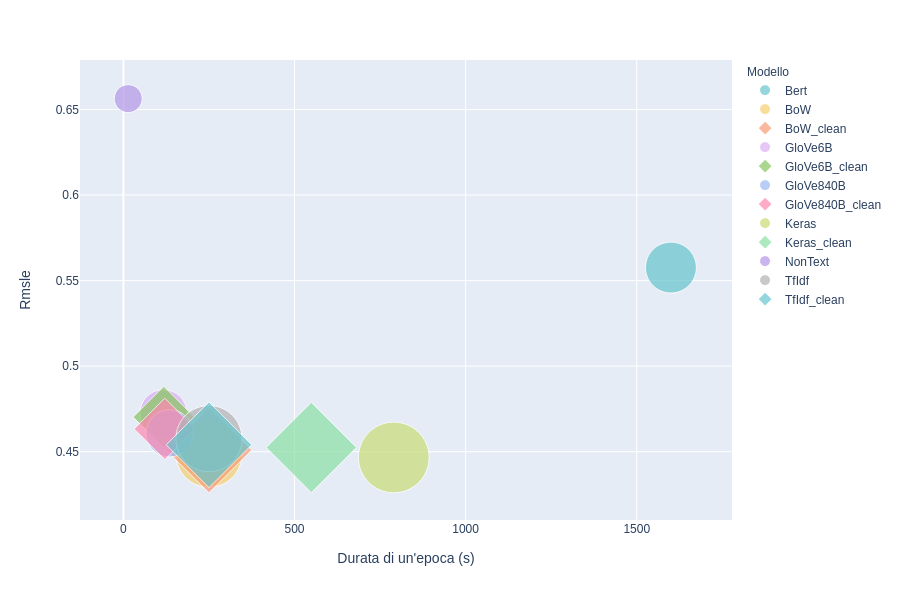
\includegraphics[
        height=6cm,
        keepaspectratio,
    ]{aml_rmsle_epocht_trainp.png}
    \caption{Rmsle sul test in funzione della Durata di un epoca di training.
        La dimensione corrisponde ai Parametri Allenabili. I risultato
        utilizzanti il preprocessing completo sono indicati da rombi.}
    \label{fig:resEtime}
\end{figure}

\begin{figure}[H]
    \centering
    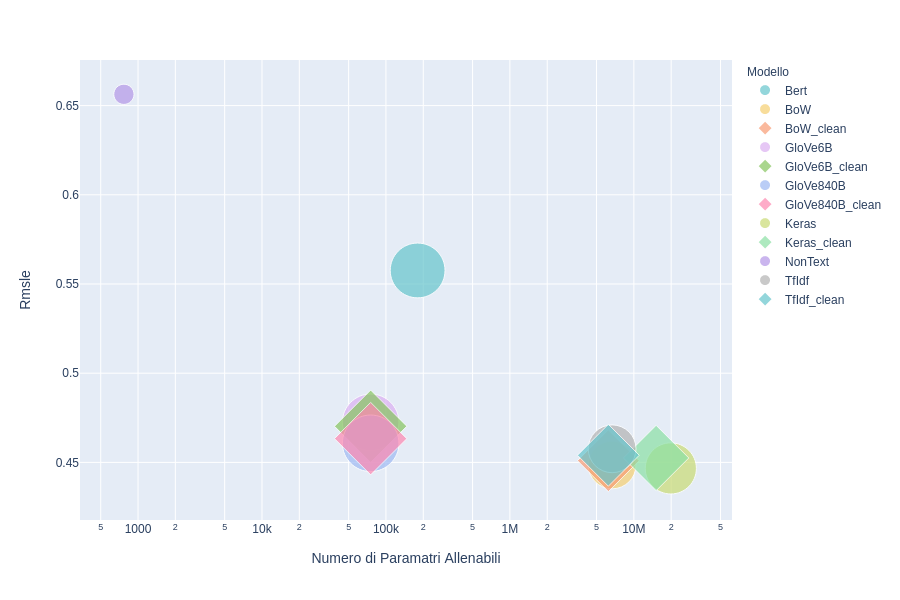
\includegraphics[
        height=6cm,
        keepaspectratio,
    ]{aml_rmsle_trainp_totp.png}
    \caption{Rmsle sul test in funzione del Numeri di Parametri Allenabili.
    La dimensione corrisponde ai Parametri Totali. I risultato
    utilizzanti il preprocessing completo sono indicati da rombi.}
    \label{fig:resParam}
\end{figure}

